\newcounter{Kcounter}
\newcommand{\sorSzamK}{\stepcounter{Kcounter}\theKcounter}

\section{Kategóriák és keresés}
\subsection{Kategóriák}
Az oldalra regisztrált szakemberek előre definiált kategóriákba kerülnek besorolásra tudásuk és végzettségeik alapján (\kovAzon{Ka\_\sorSzamK}). Egy szakember egyszerre több kategóriába is besorolható, továbbá bármilyen kombináció fennállhat a hozzájuk rendelt kategóriák között. Ezen kategóriák közül három különleges szerepet tölt be. Ezen elemek a főkategóriák és a következő névvel rendelkeznek a rendszerben (\kovAzon{Ka\_\sorSzamK}):
\begin{itemize}
     \item Tervező,
     \item Kivitelező,
     \item Műszaki ellenőr.
\end{itemize}

Minden főkategóriának vannak alkategóriái, melyek listája nincsen rögzítve, hanem bármikor bővíthető az új technológiák vagy szakmák megjelenésével. Az alkategóriák közé tartozhat például az ács, amelynek fő kategóriája a kivitelező, vagy éppen a belsőépítészeti tervező, amely pedig a Tervező kategória alkategóriája. Ezen listák bővítését csak az adminisztrátor jogú felhasználok az erre biztosított oldalon végezhetik el (\kovAzon{Ka\_\sorSzamK}). Minden alkategória hozzáadásánál pedig meg kell adniuk az adminisztrátoroknak, hogy mely főkategóriába tartozik az adott elem.


\newcounter{Szcounter}
\newcommand{\sorSzamSz}{\stepcounter{Szcounter}\theSzcounter}
\subsection{Szakemberek keresése}

A "Segítség, építkezem!" weboldalnak két kereső oldallal rendelkezik, melyek közül az egyik feladata, hogy a felhasználó megtalálja a számára legalkalmasabb szakembert/szakembereket (\kovAzon{Sz\_\sorSzamSz}). Erre több előre definiált szűrő és egy általános kereső lesz a felhasználó segítségére (\kovAzon{Sz\_\sorSzamSz}). Az előre definiált szűrökkel a szakemberek 
\begin{itemize}
     \item nevére,
     \item fő- és alkategóriákra,
     \item földrajzi helyére (megyei szinten),
     \item értékelésére,
     \item általa használt termékekre,
     \item általa nyújtott szolgáltatásokra,
\end{itemize}
tud szűkíteni a felhasználó. Míg az általános keresővel a szakember összes publikus adatai között tud keresni a felhasználó.

A keresés eredményében megjelenítésre kerül (\kovAzon{Sz\_\sorSzamSz}) egy-egy szakember
\begin{itemize}
     \item neve,
     \item profilképe,
     \item egy link a referenciáira.
\end{itemize}
A keresési eredmények rendezhetőek is a szakember értékelése, és a referenciának száma alapján (\kovAzon{Sz\_\sorSzamSz}).

\begin{figure}[h]
	\centering
	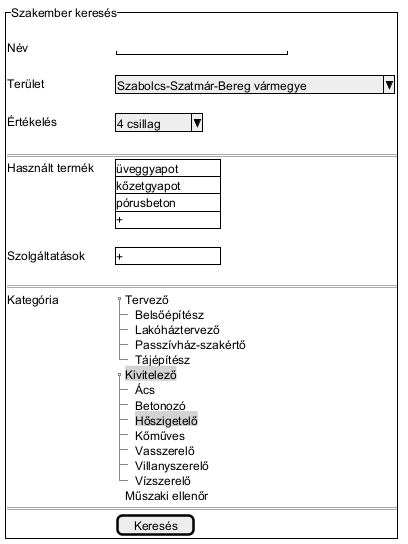
\includegraphics[scale=0.5]{img/szakember_keres.png}
	\caption*{Szakember keresése}
	\label{fig:szak_ker}
\end{figure}

\begin{figure}[h]
	\centering
	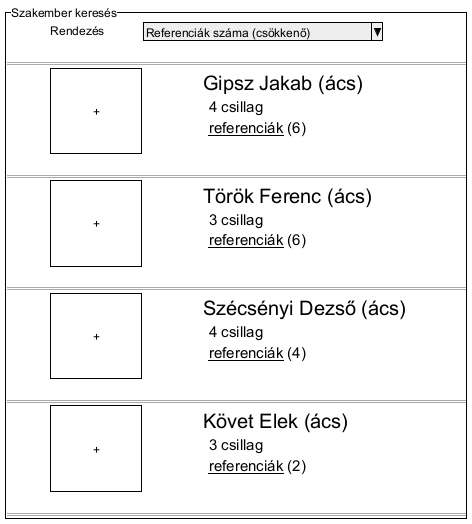
\includegraphics[scale=0.5]{img/szakember_eredmeny.png}
	\caption*{Szakember keresési eredmény}
	\label{fig:szak_ker_ered}
\end{figure}